\subsection{Representation: RTE as AST}


{  %\setbeamercolor{background canvas}{bg=sectioncolor}
\begin{frame}{\Challenge{1} RTE Representation}

  How to represent an RTE in Clojure, Scala, Python, etc...?


  \medskip
  
  %% \begin{itemize}
  %% \item Surface syntax: declarative, expressive, composable
  %% \item Programmatic interface: reflective, algebraic manipulation
  %% \end{itemize}
\end{frame}
}


\begin{frame}[t]{RTEs}{PL Declarative, Composable Syntax}
  \begin{columns}
    \begin{column}{0.55\textwidth}
  \begin{itemize}
  \item Mathematical notation:\\
  \quad\textcolor{greeny}{$(Int \cdot (Float \cup odd)^+)^*$}

  \item Leaf nodes interface to native type system

  \item \only<3>{ Scala notation:\\
    \usebox\exnoteboxscala}%
  \only<2>{ Python notation:\\
    \usebox\exnoteboxpython}%
  \only<1>{ Clojure notation:\\
    \usebox\exnoteboxclojure}%
  \end{itemize}
    \end{column}%
    \begin{column}{0.45\textwidth}
      \scalebox{0.7}{% Modeled after the following
% A simple Tree
% Author: Stefan Kottwitz
% https://www.packtpub.com/hardware-and-creative/latex-cookbook
\documentclass[border=10pt]{standalone}
\usepackage{tikz}
\begin{document}
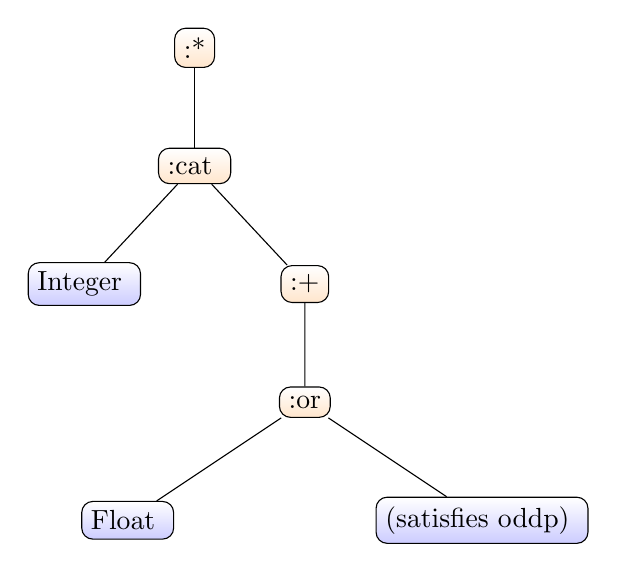
\begin{tikzpicture}[sibling distance=10em,
  every node/.style = {shape=rectangle, rounded corners,
    draw, align=center,
    top color=white, bottom color=orange!20}]]
    \tikzstyle{level 2}=[sibling distance=28mm]
    \tikzstyle{level 4}=[sibling distance=45mm]
  \node {\code{:*}}
  child { node { \code{:cat} } 
    child { node [bottom color=blue!20] {\code{Integer} } }
    child { node {\code{:+}} 
      child { node {\code{:or}}
        child { node [bottom color=blue!20] {\code{Float} } }
        child { node [bottom color=blue!20] {\code{(satisfies oddp)} } } } } } ;
\end{tikzpicture}
\end{document}
}
    \end{column}%
  \end{columns}%
\end{frame}

